\section{Experimental Results}
We now assess our CRU-FM model experimentally.
First, we study a synthetic task where we can control the missingness mechanism precisely (varying between data-dependent and data-independent). 
Second, we study extrapolation performance on 3 real open-access datasets of critical care electronic health records (EHR).

%as well as on thre large open-access datasets of critical care electronic health records (EHR): Physionet(specifically the computing in cardiology challenge 2012 \citep{silva2012predicting}) and MIMIC-IV \citep{johnson2020mimic}. 


We compare to 6 total competitive baselines for irregular time series modeling.
First, 
\citet{schirmer2022modeling}'s CRU model (Sec.~\ref{sec:CRU_gen_model_from_prev_work}) is a natural baseline, as it represents removing the data-dependent missingness mechanism of our CRU-FM.
Additionally, we compare to 
 mTAND \citep{shukla2021multitime}, pVAE \citep{li2020learning},
 Latent ODE~\citep{rubanova2019latent}, and Neural CDE~\citep{kidger2020neural}. 
On the synthetic task, we also compare to an additional recent LLM baseline for time series forecasting called LLMTime \citep{gruver2023large}. Due to its poor performance, we did not apply it to any EHRs.
%on this toy task, we did not spend time applying this baseline to later large EHR datasets.


\subsection{Synthetic Experiments}
\label{sec:synthetic_experiment}


\textbf{Purpose.}
We designed a synthetic extrapolation task with $D{=}2$ data channels to assess how well each model can learn from hundreds of sequences drawn from a known data-generating process that includes data-dependent missingness (defined in equations \ref{eq:gen_data_toy_eq} and \ref{eq:seen_proba_toy}).
Figure~\ref{fig:toy_example_sequences} illustrates two example sequences.
The top channel is a square wave with a sequence-specific phase offset.
The bottom channel is a sinusoid whose amplitude and phase depend on the  current value of the top channel.  
As detailed below, our data-generation process introduces missingness in a channel at different rates depending on whether the channel's current value is inside or outside the illustrated blue horizontal bounds. 

This process results in significant missingness in the top (first) channel. Thus, in order to deliver good extrapolations for both channels, a model must accurate model dependencies in feature values and missingness jointly across channels.

\textbf{Setup.}
To generate each sequence (indexed by $n$), we draw a horizontal offset $b_n \sim \text{Unif}([0,2])$. 
This value informs a deterministic ``true'' time-varying data-generation function $x_{n,d}(t)$ for each dimension $d$: we have a square wave for $d=1$ and a sine wave for $d=2$ 
\begin{align}
    x_{n,1}(t) &= \operatorname{sgn}(\sin(4\pi t+b_n))
    \\ \notag 
    x_{n,2}(t) &= \sin(4\pi t+b_n) \cdot x_{n,1}(t)
    + 0.4 \cdot \cos(4\pi t+b_n) \cdot (1-x_{n,1}(t))
\label{eq:gen_data_toy_eq}
\end{align}

For each sequence $n$, a set $\Gamma_n$ of observation times is drawn with 50 elements, each one i.i.d. uniform within $(0, 2)$. At each time $t \in \Gamma_n$, the indicator controlling whether dimension $d$ is seen or missing is then sampled so that inside the blue lines of Fig.~\ref{fig:toy_example_sequences}, there is a good chance of observation (60\%), but outside the lines the chance is lower:
\begin{align}
     p( s_{ntd} = 1 ) =
 \begin{cases}
 0.6 & \text{if } -0.4 < x_{n,d}(t) < 0.4 \\
 p_{\text{S}} & \text{otherwise }
 \end{cases}    
 \label{eq:seen_proba_toy}
\end{align}
Here, scalar $p_{\text{S}} {>} 0$ determines the chance of seeing an outside-the-lines value. By default, we fix $p_{\text{S}} {=} 0.0006$, yielding a data-dependent missingness mechanism for both channels. 
Later sensitivity analyses study what happens as $p_{\text{S}}$ increases toward 0.6 (MCAR scenario).


\textbf{Extrapolation task.}
We generated 1000 sequences (keeping only the $x_{nt}, s_{nt}$ values at times in $\Gamma_n$), divided into train/valid/test splits of size 700/150/150. 
After training and tuning any model, we measure extrapolation on each test sequence by providing data up to time $t=1.5$, then obtaining from each model the \emph{most likely} predicted value for each channel at each heldout time in $(1.5, 2.0)$.



%  The MNAR conidtion is as follows : 
% \[
% p(s_{n,k}(t)=1|f_{n,k}(t)) =
% \begin{cases}
% 0.6 & \text{if } -0.4 < f_{n,k}(t) < 0.4 \\
% 0.0006 & \text{otherwise }
% \end{cases}
% \]
% where $s_{n,k}(t)$ is an indicator for observing data in the $k^{th}$ channel of the $n^{th}$ sequence at time $t$. $s=1$ if data is observed and 0 otherwise. 2 example sequences are shown in figure \ref{fig:toy_example_sequences}. We generate 800 sequences and divide the train/valid/test splits as 500/150/150. We choose the best model as the one with the lowest validation mean-squared-error in the extrapolated segment (highlighted by dashed lines at $t>1.5$ in figure \ref{fig:models_generated_seq}).



\begin{figure*}[!ht]
\centering
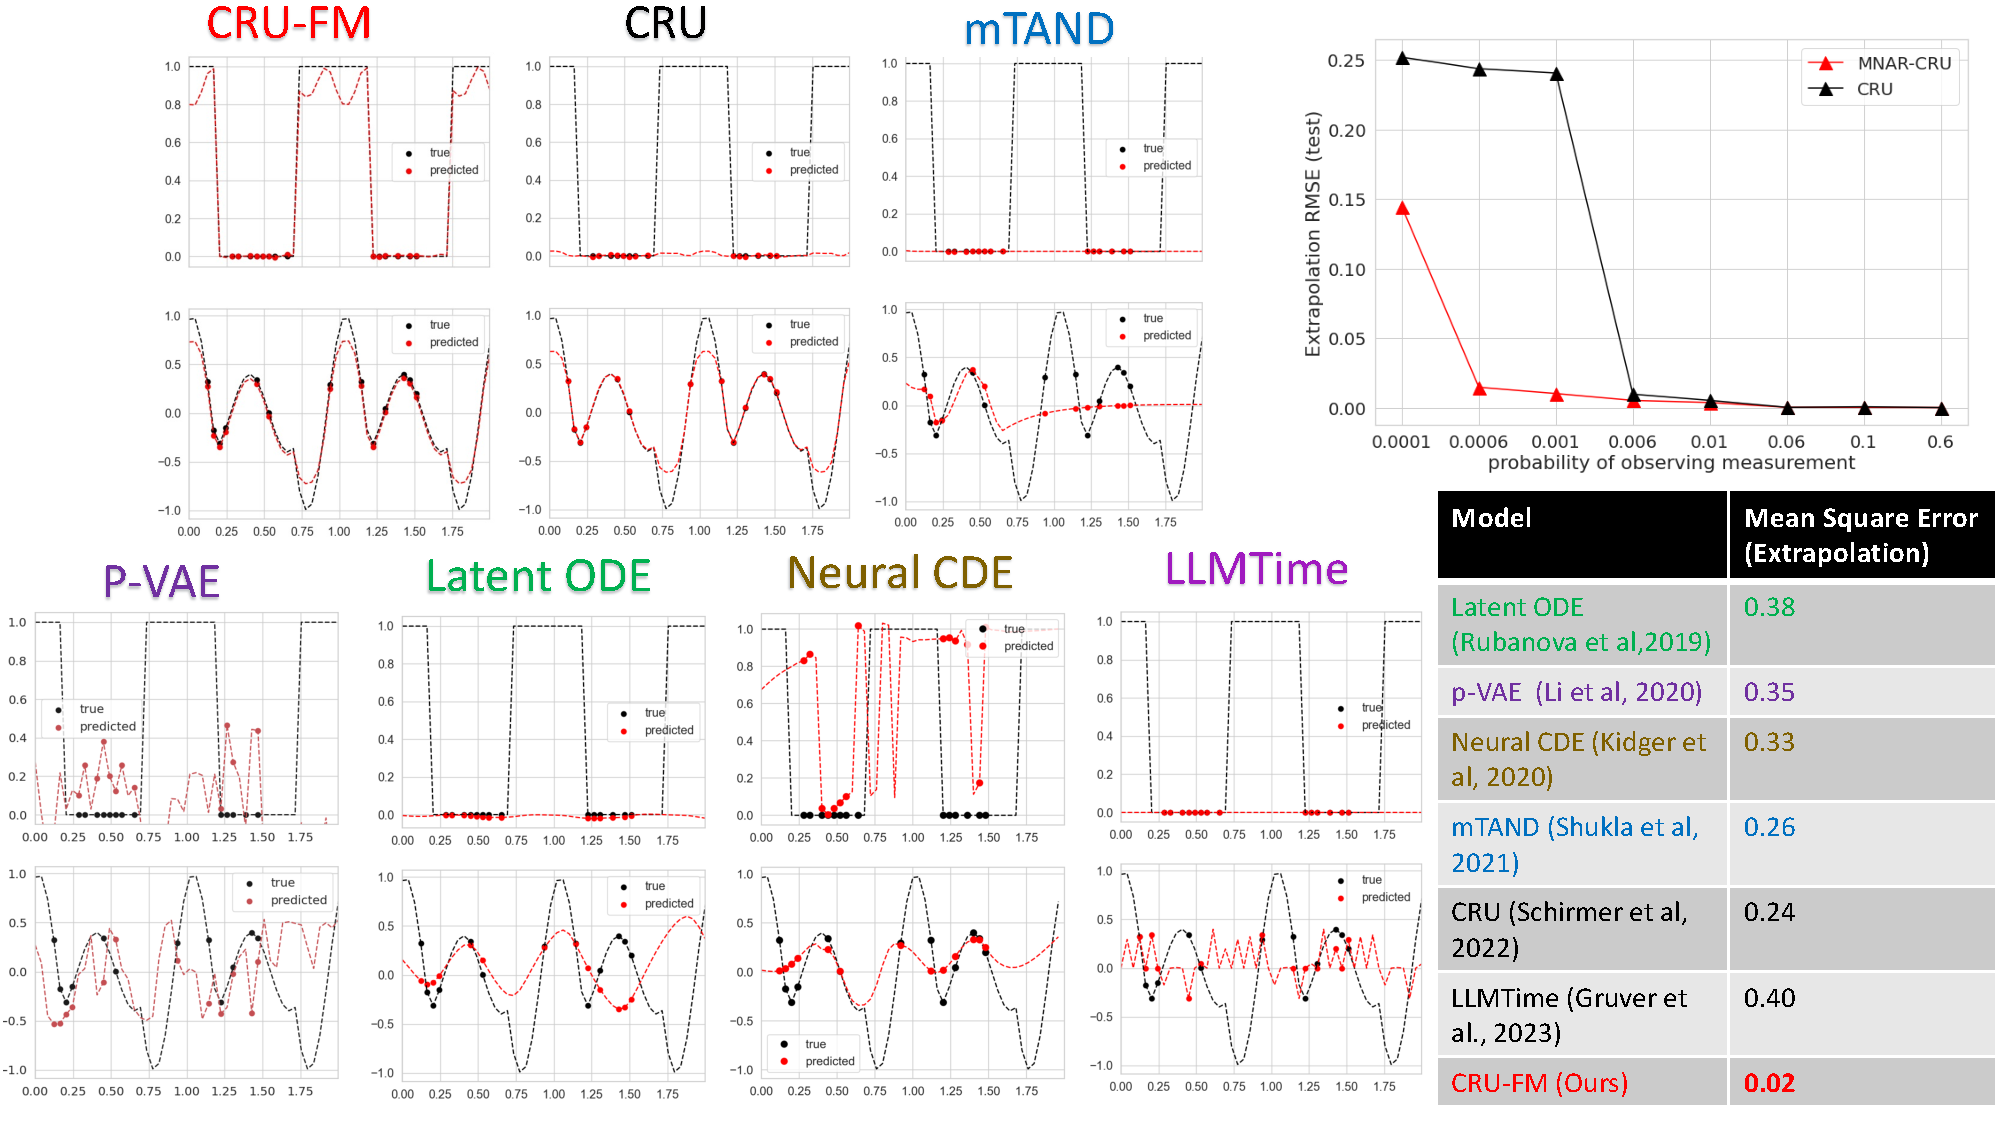
\includegraphics[width=1.0\textwidth]{content/chapters/irregular_time_series_data_driven_missingness/figures/toydata_extrapolation_improved.pdf}
\caption[Synthetic task results comparing CRU-FM to competitors]{Synthetic task results comparing CRU-FM to competitors.
\emph{Left:} Visuals of reconstruction ($t \in (0, 1.5)$) and extrapolation ($t \in (1.5, 2)$) for the \emph{same} 2-channel test sequence when missingness is data-dependent ($p_{\text{S}} {=} 0.0006$).
Black (red) lines indicate true (reconstructed) values. To fairly compare models, we evaluate each one's most likely prediction $\hat{x}_{t}$ (mode of the predictive distribution). 
For example, for our CRU-FM we set $\hat{x}_{t} = h_{t}$ (via Eq.~\eqref{eq:mnar_cru_model}).
This choice eliminates extraneous randomness needed to sample from a predictive distribution.  \emph{Bottom Right:}
Extrapolation results on the synthetic task sequences comparing MNAR-CRU, CRU, MTAND and p-VAE. The black/red dots are the observed/predicted values at each irregularly sampled time point. The black/red line is the true/reconstructed sequence. Each model is trained until $t=1.5$ and the extrapolated from $t=1.5$ to $t=2$. MNAR-CRU generates sequences that are closer to the ground-truth and also achieves the least mean squared error on the extrapolation task. We attribute this improved performance of the MNAR-CRU to the model's ability to learn the true missingness probability in each sequence. \textit{Top right :} We examine how extrapolation error changes as the probability of observing a measurement (denoted as $p_{obs}$) outside the (-0.4, 0.4) bounds changes. As $p_{obs}$ increases (MNAR assumption relaxes), as expected the CRU and MNAR-CRU perform similarly. For low values $p_{obs} \leq 0.006$, MNAR-CRU’s better-specified missingness model notably improves extrapolation (via a joint model of $x_t$ and $s_t$).
}%endcaption
\label{fig:models_generated_seq}
\end{figure*}

\textbf{Results: Head-to-head comparison with competitor models :}
Fixing $p_{\text{S}} = 0.0006$ to ensure data-dependent missingness, we compare the extrapolation error of our CRU-FM with all competitors.
In the lower right panel of Fig.~\ref{fig:models_generated_seq},
CRU-FM delivers by far the lowest overall mean squared error on the test set of 150 sequences (0.02 vs. 0.24 for the next best competitor, the CRU). 

To understand possible reasons for CRU-FM's improved performance, we show plots of sequence-specific reconstructions/extrapolations from each model 
(left panels of Fig.~\ref{fig:models_generated_seq}).
These plots confirm CRU-FM recovers the underlying ``true'' model structure best, especially looking at the more difficult first (top) channel.
All models are trained on the same 700 sequences, few of which do have rare cases of observations from the top of the square wave. 
We suggest our model handles this top channel better than alternatives because it is the only tested model capable of data-dependent missingness. 
CRU-FM's
 latent representations $\mu_t$ are informed by both features $x_t$ and seen/missing indicators $s_t$, enabling learning of dependencies between channels (e.g. steep slope in channel 2 is indicative of a crest in channel 1 even when channel 1 is often missing). 
%ltimately resulting in superior extrapolative performance.

%It's important to note that data points are not $100\%$ missing at the crest of the square-wave but have a very low probability of observation: 0.0006. Given that our training involves 700 sequences drawn from the same process (see Fig 2 and the equation below it), the model does encounter a number of sequences that include observations in the crest/peak of the square wave. Thanks to our joint model, the variables \(x_t\) and \(s_t\) are informed by posterior means (\(\mu_t^+\)), enabling learning of dependencies between channels (e.g. steep slope in channel 2 is indicative of a crest in channel 1, ultimately resulting in superior extrapolative performance.

As illustrated in Fig.~\ref{fig:models_generated_seq}, 
the second (bottom) channel is extrapolated similarly well by both the CRU and the CRU-FM, both much better than other models.
We suggest two possible reasons CRU is similar to CRU-FM on this channel.
First, channel 2 spends less time outside the (-0.4, 0.4) bounds and is thus typically observed.
Second, unlike the sharp jump of the square wave in channel 1, the true function of channel 2 transitions \textit{smoothly} across the (-0.4, 0.4) bounds, so sane extrapolations are possible even for simpler models.

\textbf{Results: Sensitivity analysis to missingness mechanism.}
To further verify that capturing the data-dependent missingness of our model is the primary reason for success,
we sweep $p_{\text{S}}$ from 0.0006 to 0.6 (MCAR). At each value,
we resample all train/valid/test data and retrain the CRU-FM and CRU. As expected, the top-right panel in Fig.~\ref{fig:models_generated_seq} shows that our CRU-FM yields far lower error in the data-dependent missingness setting, but becomes indistinguishable from the CRU in the MCAR setting. This helps rule out other confounding explanations for which model is superior, like better tuning or lucky initialization.


\textbf{Results : Parameter Learning on Toy Data}
We show the capability of our model to learn the missingness parameter for each channel in our toy example in figure \ref{fig:learning_missingness_mechanism}
\begin{figure}[h]
    \centering
    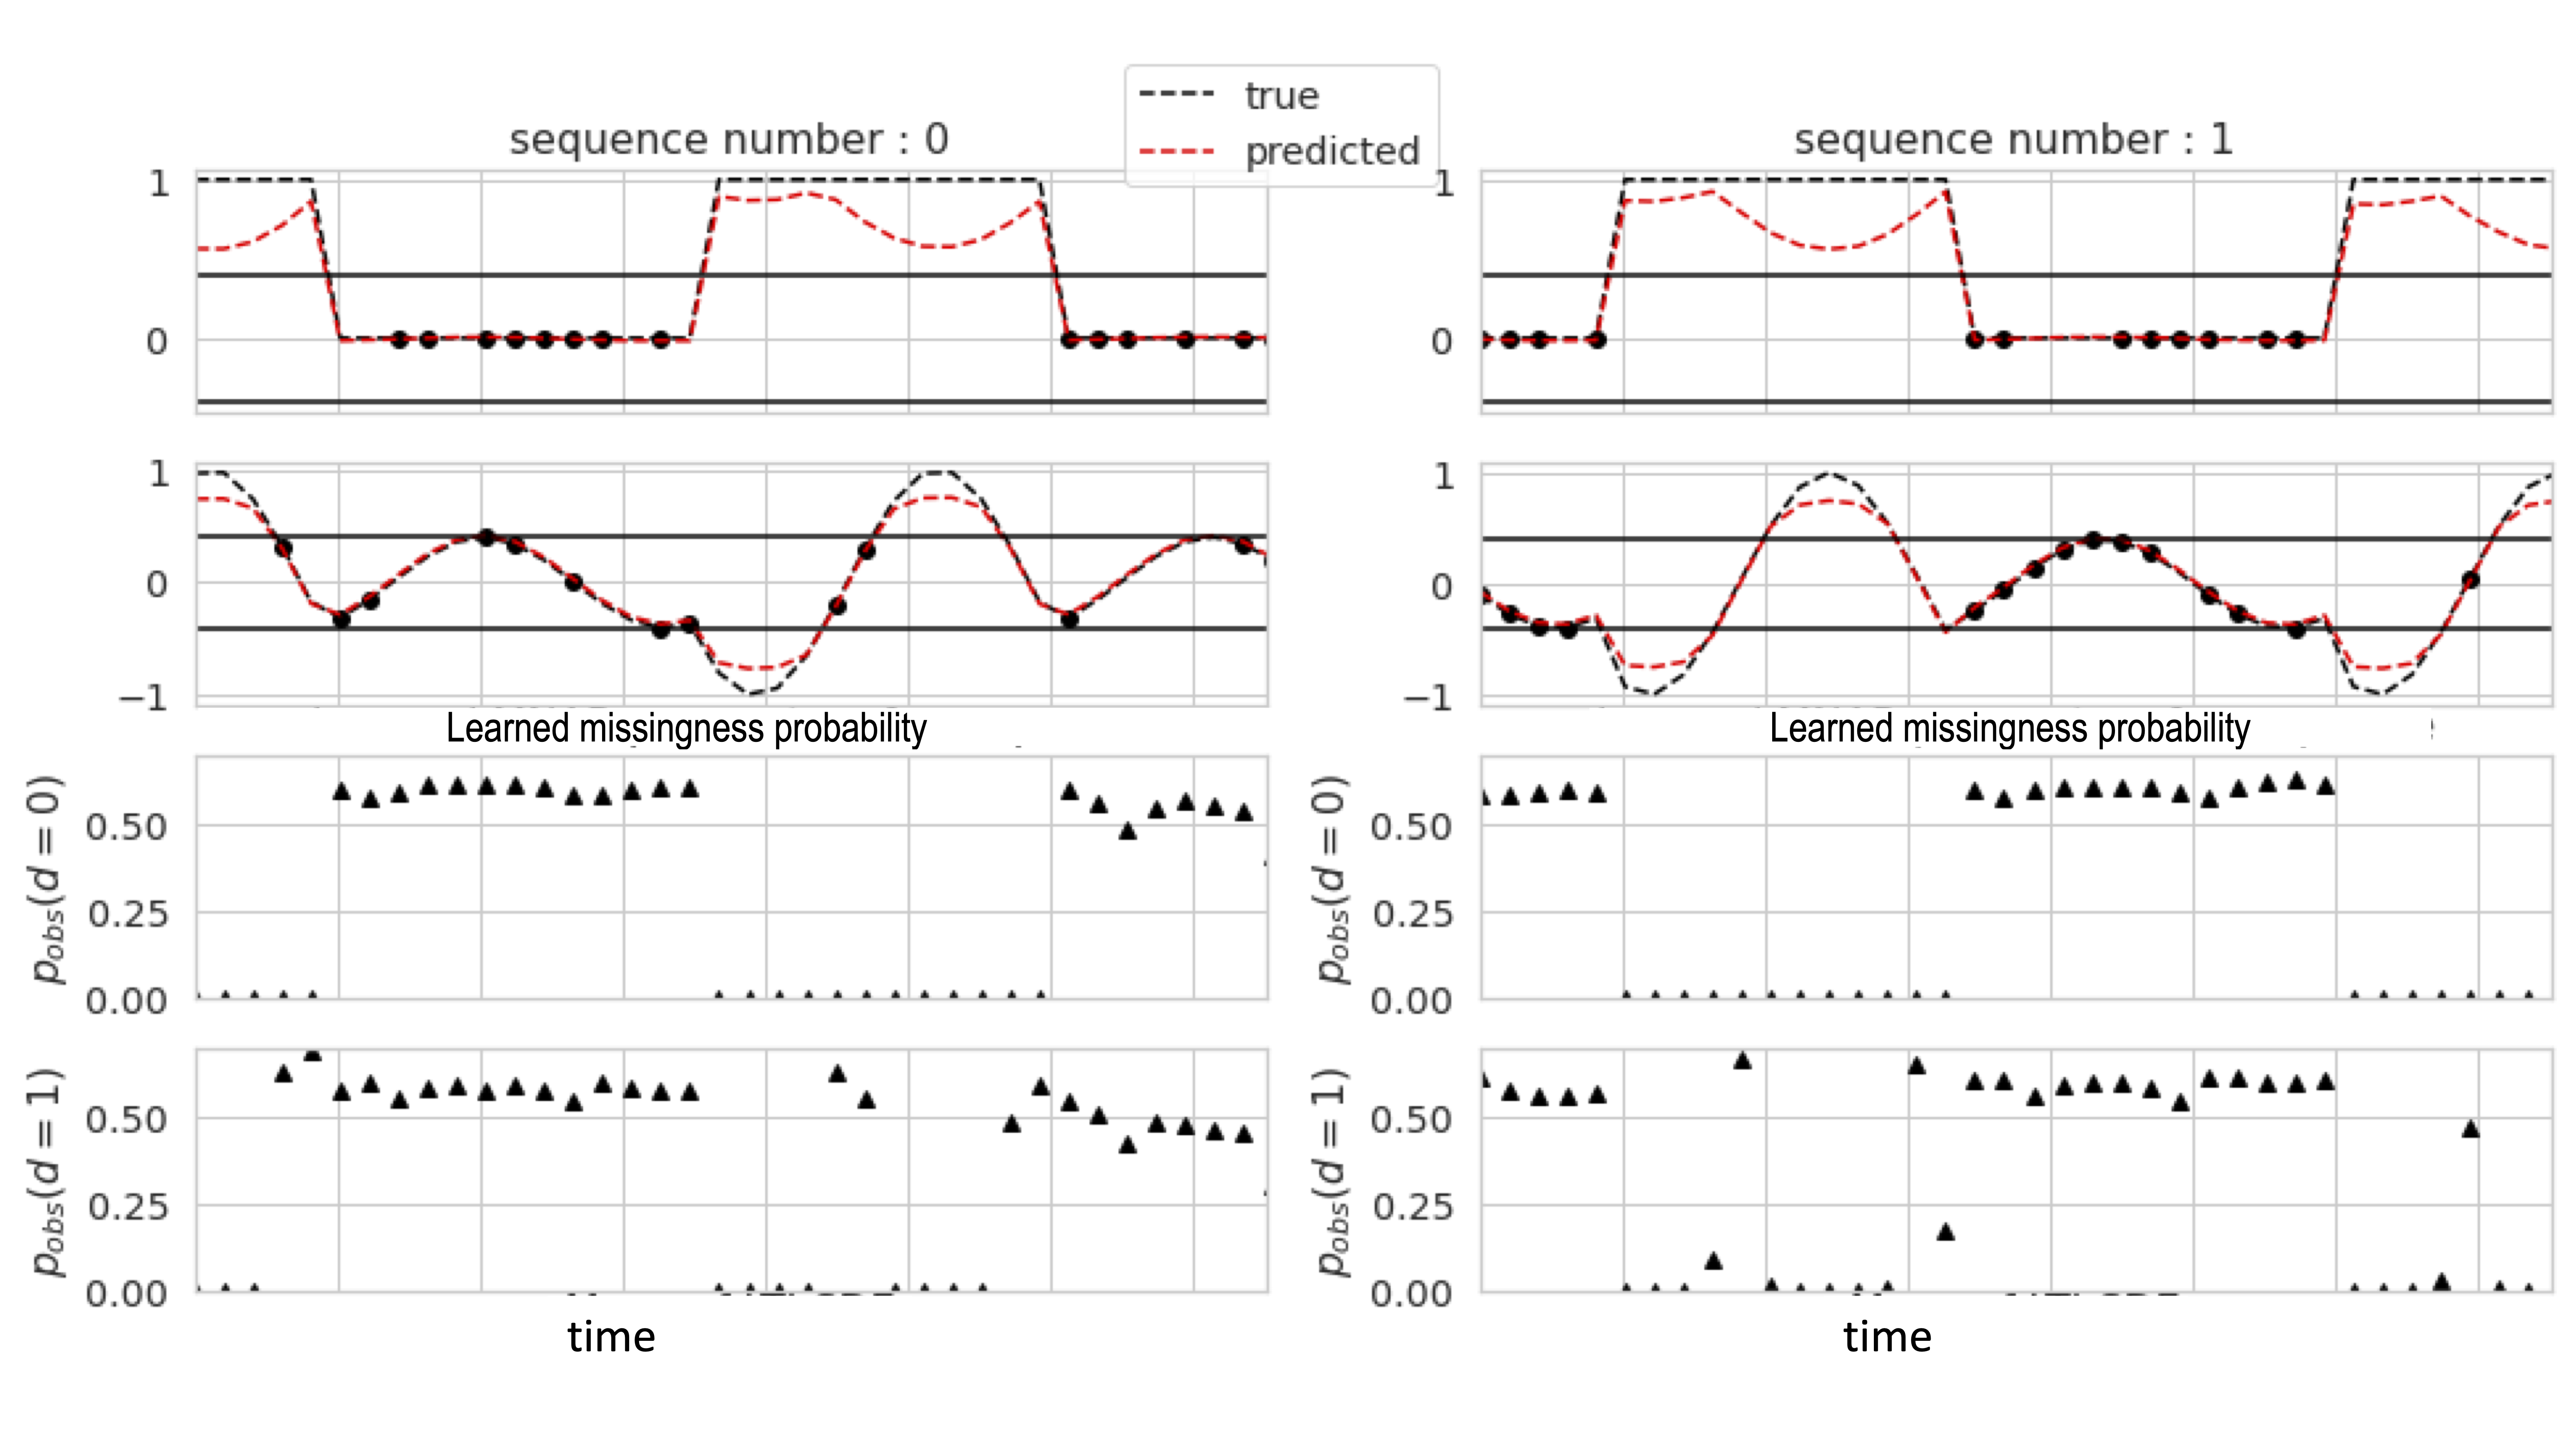
\includegraphics[width=1.0\textwidth]{content/chapters/irregular_time_series_data_driven_missingness/figures/learning_mnar_mechanism.png}
    \caption[Demonstration of our CRU-FM model’s ability to learn the data-dependent missingness mechanism]{Demonstration of our CRU-FM model's ability to learn the data-dependent missingness mechanism. \textit{Top 2 rows : } We show the 2 channels of data from 2 representative sequences from our toy experiment (details in section \ref{sec:synthetic_experiment}). The black dashed line and the red dashed line represent the true and reconstructed sequences respectively. The black dots represent the observed values at irregularly spaced timepoints. \textit{Bottom 2 rows : } Learned probabilities of observing a measurement in each of the channels above.
    Remember, we set the data-dependent missingness mechanism as follows : the probability of observing a value outside the dashed black lines for each channel is 0.0006 and the probability of observing a measurement within the dashed black lines is 0.6. This mechanism is learned by our model (the black upward arrows show the learned probabilities of observing a value). The ability of our model to learn these data-dependent missingness mechanisms leads to improved downstream extrapolation performance.}
    \label{fig:learning_missingness_mechanism}
\end{figure}


\subsection{Results on Real EHR Datasets}
Next, we examine extrapolation error when trained models from different competitor methods get to observe the first 24 hours of patient health-records (labs and vitals) then must extrapolate the same measurements over the next 6-24 hours. We evaluate on 3 separate large EHR datasets that are all de-identified and publicly available.

\textbf{Physionet-2012 setup.} 
The Physionet-2012 challenge dataset \citep{silva2012predicting} is available at \href{https://physionet.org/content/challenge-2012/1.0.0/.}{https://physionet.org/content/challenge-2012/1.0.0/}. 
%contains 8000 ICU stays.
We only include 8000 ICU stays lasting at-least 48 hours and exclude static measurements, following earlier analyses by \citet{rubanova2019latent}.
For each stay, we model all 37 labs and vitals available in released data (see Tab.~\ref{tab:physionet_features} for feature details and missingness rates).
Our train/valid/test splits have 4800/1600/1600 patient stays.
\begin{table}[!ht]
    \centering
    \begin{tabular}{|c|c|c|c|} \hline 
         Feature&  Min&  Max& Observation rate per hour  (averaged over first 48 hours)\\ \hline 
         Weight&  0.0&  300& 0.640\\ \hline 
         Albumin&  0.00&  4.70& 0.012\\ \hline 
         ALP&  0&  1024& 0.016\\ \hline 
         ALT&  0&  11030& 0.016\\ \hline 
         AST&  0&  16200& 0.016\\ \hline 
         Bilirubin &  0&  45.8& 0.016\\ \hline 
         BUN&  0&  170& 0.071\\ \hline 
         Cholesterol&  0&  240& 0.002\\ \hline 
         Creatinine&  0&  16& 0.072\\ \hline 
 DiasABP& 0& 268&0.768\\ \hline 
 FiO2& 0& 1&0.170\\ \hline 
 GCS& 0& 15&0.327\\ \hline 
 Glucose& 0& 1075&0.067\\ \hline 
 HCO3& 0& 42&0.070\\ \hline 
 HCT& 0& 61.8&0.095\\ \hline 
 HR& 0& 211&1.170\\ \hline 
 K& 0& 9.4&0.075\\ \hline 
 Lactate& 0& 31&0.043\\ \hline 
 Mg& 0& 7.7&0.070\\ \hline 
 MAP& 0& 300&0.757\\ \hline 
 Mechvent& 0& 1&0.162\\ \hline 
 Na& 0& 165&0.070\\ \hline 
 NiDiasABP& 0& 161&0.497\\ \hline 
 NIMAP& 0& 165.3&0.493\\ \hline 
 NiSysABP& 0& 296&0.500\\ \hline 
 PaC02& 0& 98&0.122\\ \hline 
 Pa02& 0& 500&0.121\\ \hline 
 pH& 0& 187&0.127\\ \hline 
 platelets& 0& 1047&0.074\\ \hline 
 RespRate& 0& 95&0.277\\ \hline 
 Sa02& 0& 100&0.041\\ \hline 
 SysABP& 0& 278&0.768\\ \hline 
 Temp& -17.8& 42.2&0.454\\ \hline 
 TroponinI& 0& 46.2&0.002\\ \hline 
 TroponinT& 0& 24.9&0.010\\ \hline 
 Urine& 0& 11000&0.713\\ \hline 
 WBC& 0& 528&0.067\\ \hline
    \end{tabular}
    \caption{List of features for Physionet}
    \label{tab:physionet_features}
\end{table}


\textbf{MIMIC-IV setup.} 
 Out of single-hospital MIMIC-IV dataset \citep{johnson2020mimic}, we select 
 43,883 ICU stays that last at least 30 hours.
For each stay, we track 37 time-varying labs and vitals used in prior works \citep{Gong, Nestor} (see Tab.~\ref{tab:mimic_features} for feature missingness details).
Our train/valid/test splits have 28084/7022/8777 patient-stays. 
\begin{table}[!ht]
    \centering
    \begin{tabular}{|c|c|c|c|} \hline 
         Feature&  Min&  Max& Observation rate per hour  (averaged over first 48 hours)\\ \hline 
         CRP&  0.4&  286& 0.0005\\ \hline 
         Bilirubin (direct)&  0.1&  19.7& 0.0015\\ \hline 
         Venous CO2 pressure&  20&  97& 0.008\\ \hline 
         Fibrinogen&  71.39&  792.22& 0.008\\ \hline 
         Glucose (blood)&  68&  313& 0.024\\ \hline 
         pH (venous)&  7.09&  7.53& 0.011\\ \hline 
         Height&  135&  193& 0.012\\ \hline 
         Albumin&  1.7&  4.5& 0.008\\ \hline 
         TroponinT&  0.01&  10.40& 0.011\\ \hline 
 Resp rate& 8& 35&0.014\\ \hline 
 Pa02& 51& 478&0.037\\ \hline 
 PaC02& 22& 78&0.037\\ \hline 
 pH (Arterial)& 7.09& 7.53&0.039\\ \hline 
 Bilirubin (total)& 0.2& 25.28&0.016\\ \hline 
 AST& 10& 6958.04&0.016\\ \hline 
 ALT& 5& 5200&0.016\\ \hline 
 Weight& 43.4& 158.9&0.014\\ \hline 
 Lactic acid& 0.6& 15&0.033\\ \hline 
 PT& 10.2& 52.7&0.043\\ \hline 
 Calcium& 6.5& 10.4&0.056\\ \hline 
 Phosphorus& 1.2& 9.0&0.056\\ \hline 
 Magnesium& 1.3& 3.2&0.060\\ \hline 
 ABP (systolic)& 78& 178&0.700\\ \hline 
 ABP (diastolic)& 34& 110&0.700\\ \hline 
 Temperature& 35.4& 38.6&0.220\\ \hline 
 Glucose (serum)& 63& 399&0.061\\ \hline 
 Platelets& 23& 570&0.060\\ \hline 
 Hemoglobin& 6.3& 15.2&0.070\\ \hline 
 Creatinine& 0.4& 8.7&0.060\\ \hline 
 Hematocrit& 19.4& 45.2&0.070\\ \hline 
 Potassium& 2.9& 6.4&0.070\\ \hline 
 HCO3& 10& 37&0.060\\ \hline 
 Chloride& 85& 121&0.070\\ \hline 
 Sodium& 120& 154&0.070\\ \hline 
 Resp Rate& 8& 35&0.950\\ \hline 
 O2 sat& 88& 100&0.940\\ \hline 
 Heart rate& 49& 133&0.960\\ \hline
    \end{tabular}
    \caption{List of features for MIMIC-IV}
    \label{tab:mimic_features}
\end{table}


\begin{figure}[!hp]
    \centering
    \begin{tabular}{l c c c}
        \rotatebox{90}{\hspace{3em}MIMIC-IV} 
        &
        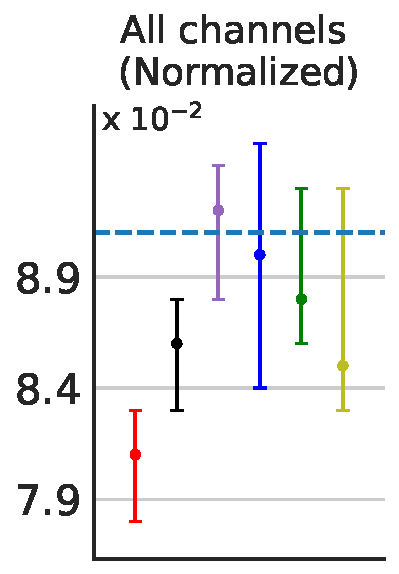
\includegraphics[height=5.2cm]{content/chapters/irregular_time_series_data_driven_missingness/figures/mimic_evaluation_summary.pdf} 
        &
        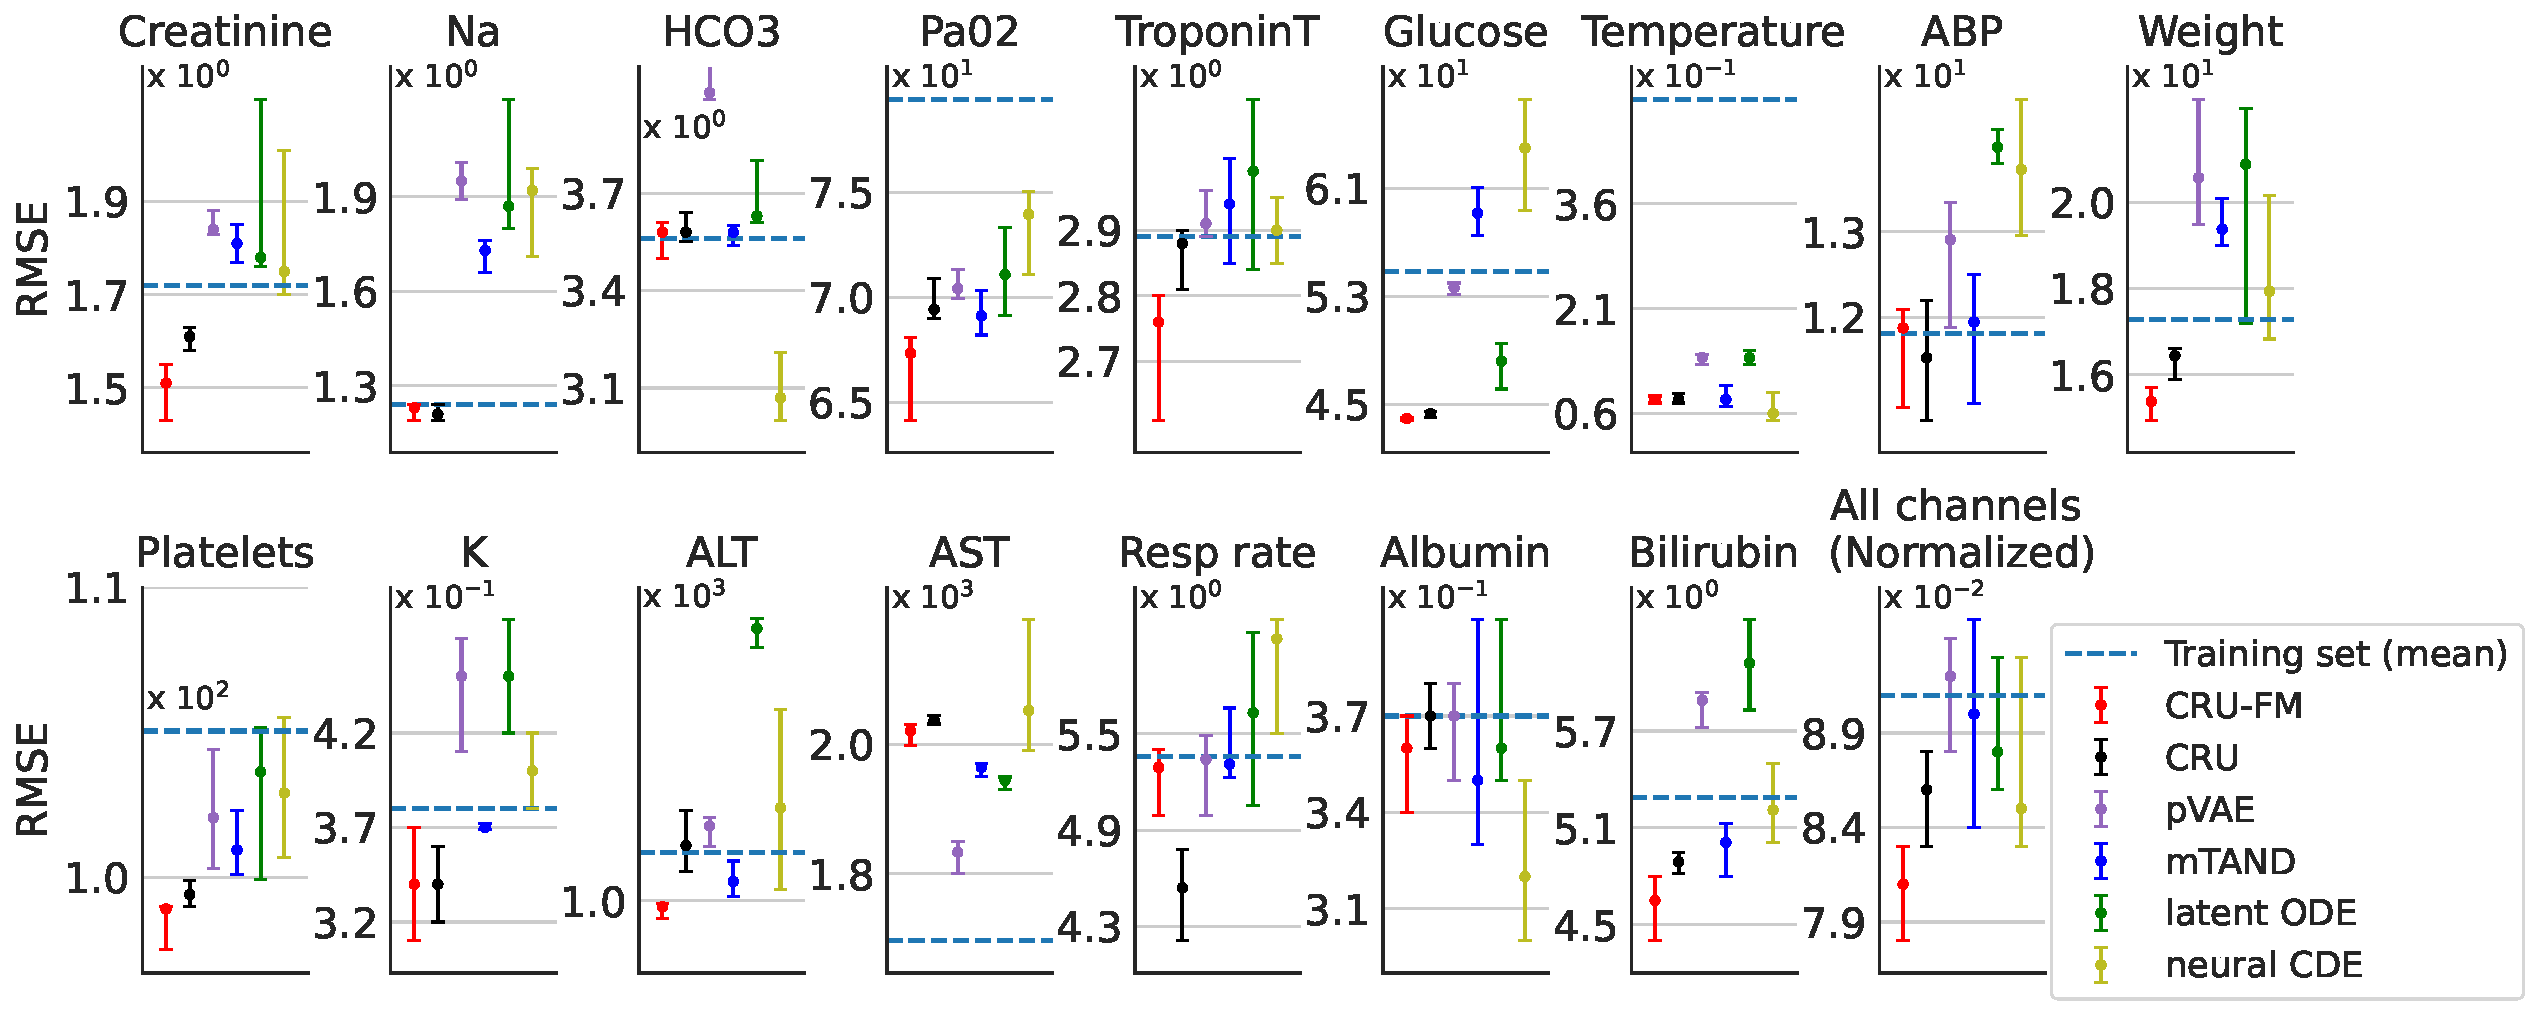
\includegraphics[trim={0 0 590 0},clip,height=5.2cm]{content/chapters/irregular_time_series_data_driven_missingness/figures/mimic_evaluation.pdf} 
        &
        \raisebox{1.5cm}{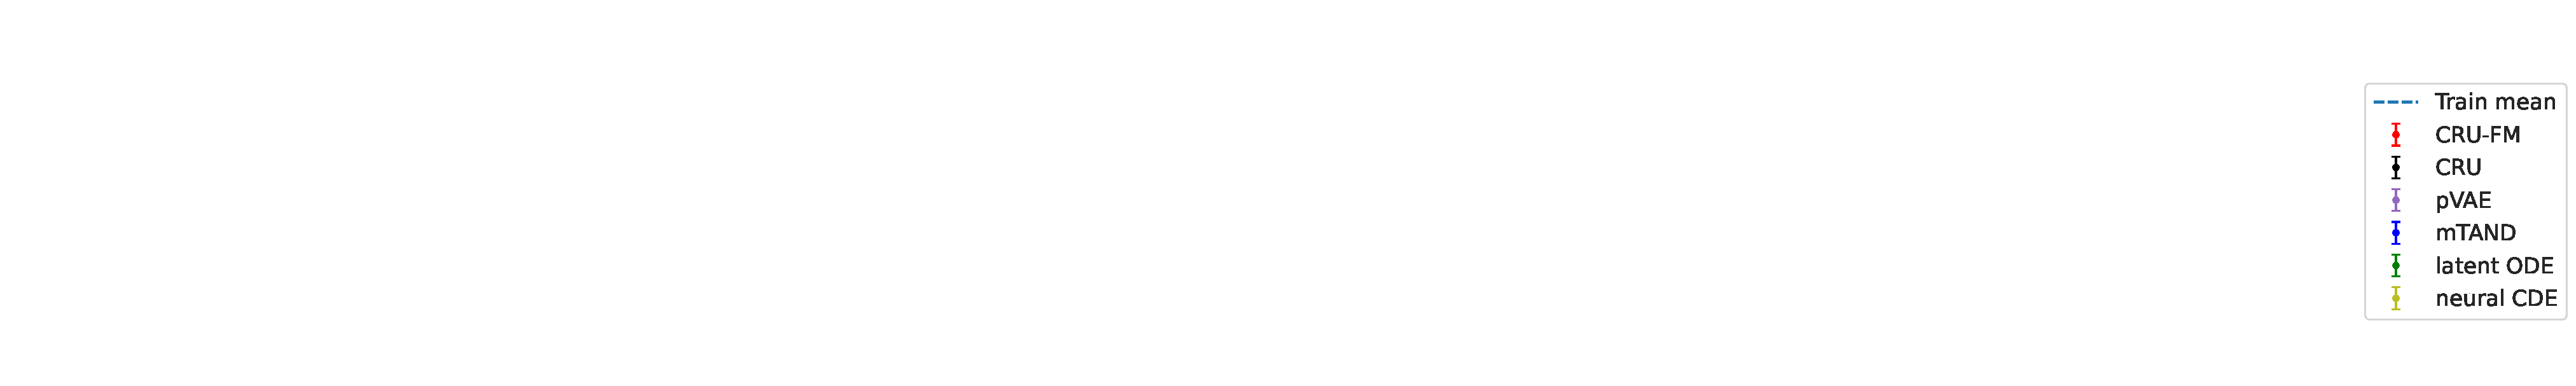
\includegraphics[height=3.5cm]{content/chapters/irregular_time_series_data_driven_missingness/figures/legend.pdf}}
    \\~\\
        \rotatebox{90}{\hspace{4em} Physionet} 
        & 
        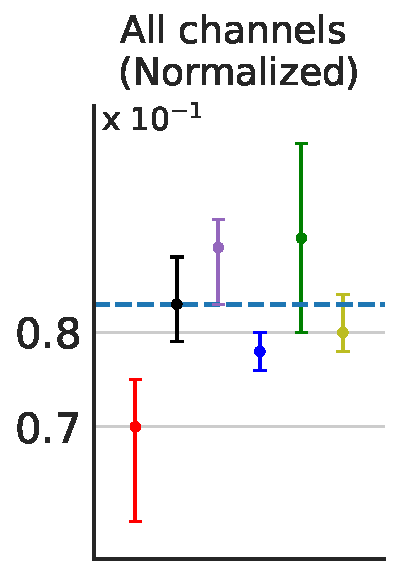
\includegraphics[height=5.2cm]{content/chapters/irregular_time_series_data_driven_missingness/figures/physionet_evaluation_summary.pdf} 
        &
        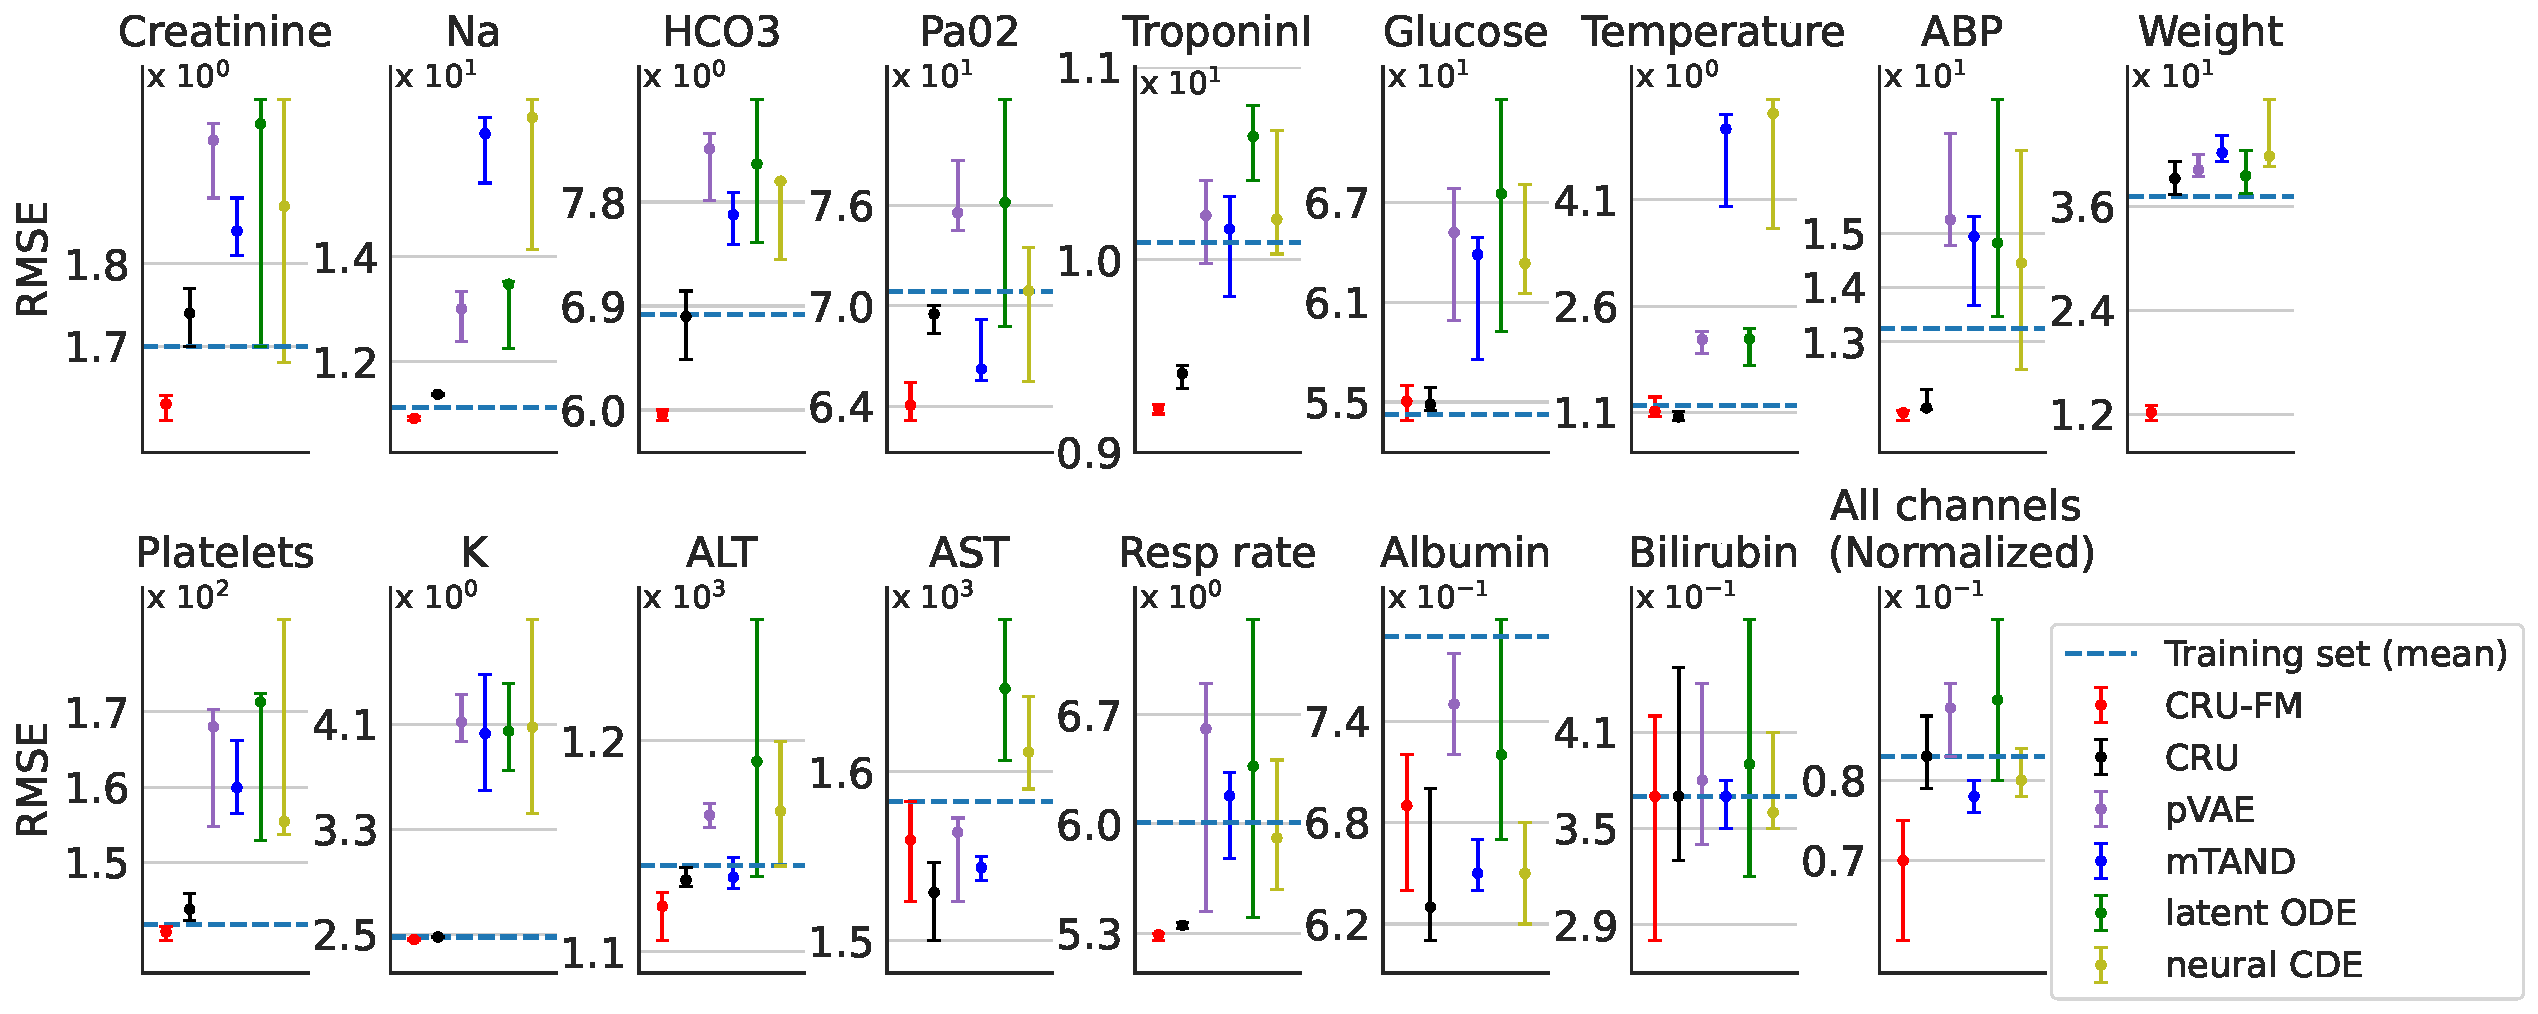
\includegraphics[trim={0 0 590 0},clip,height=5.2cm]{content/chapters/irregular_time_series_data_driven_missingness/figures/physionet_evaluation.pdf}
    \\~\\
        \rotatebox{90}{\hspace{4em} eICU}
        &
        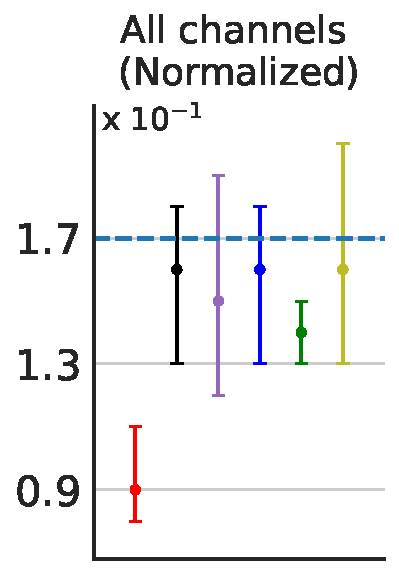
\includegraphics[height=5.2cm]{content/chapters/irregular_time_series_data_driven_missingness/figures/eicu_evaluation_summary.pdf} 
        &
        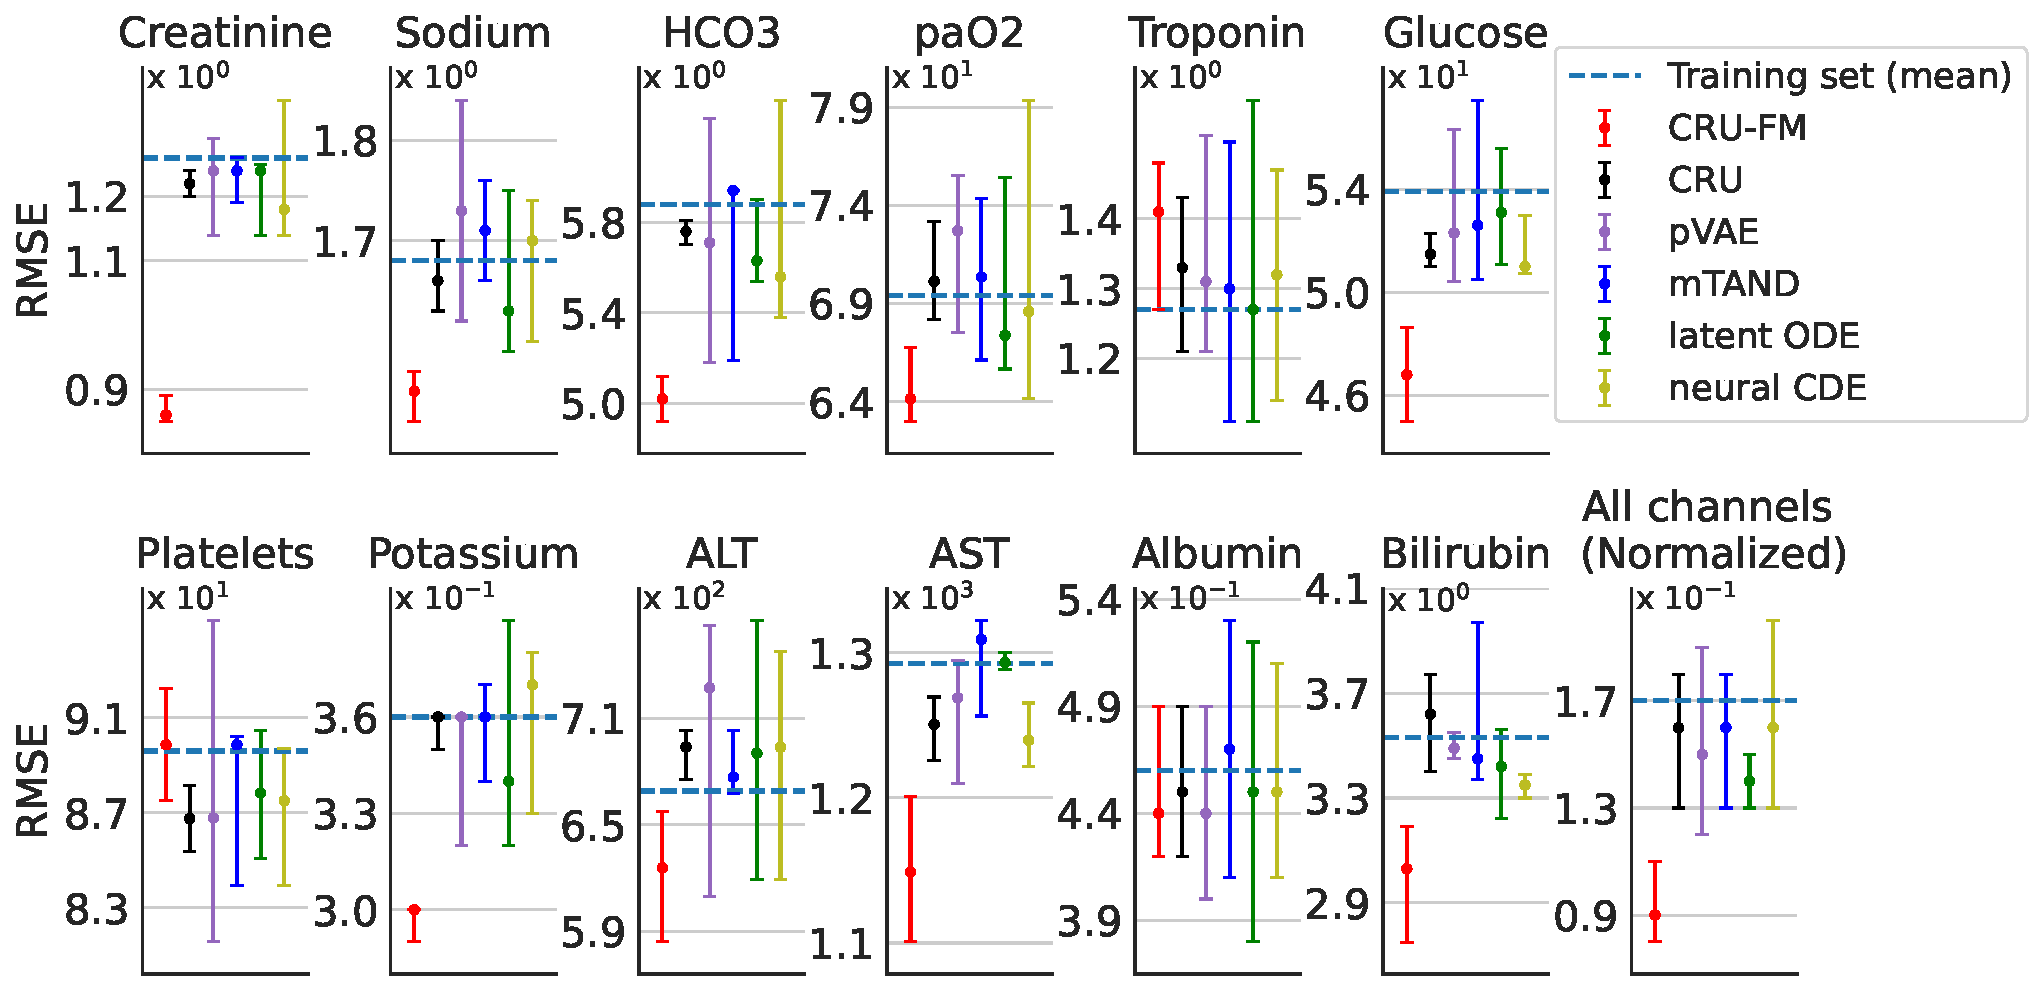
\includegraphics[trim={0 0 355 0},clip,height=5.2cm]{content/chapters/irregular_time_series_data_driven_missingness/figures/eicu_evaluation.pdf}
    \end{tabular}
    \caption[Comparison of extrapolating measurements with our CRU-FM v/s 5 competitor methods on 3 EHR datasets]{Comparison of our CRU-FM with 5 competitor methods, in terms of extrapolation error (RMSE, lower is better) on MIMIC-IV, Physionet, and eICU test sets. For each test patient-stay, the first 24 hours of data are provided as input, and methods must extrapolate the next 6-24 hours of available measurements. Confidence intervals show the 5th and 95th percentiles of the mean RMSE across 100 bootstrapped samples of the test set. 
    Our CRU-FM clearly outperforms competitors in overall error across all channels (left column). Per-channel error comparisons (right columns) for select channels also show clear wins in a majority of cases (CRU-FM's confidence interval is lower and does not overlap with others). Expanded per-channel results for all datasets in App. Fig. \ref{fig:all_channels_evaluation_extended}  
    }%endcaption
    \label{fig:real_data_evaluation}
\end{figure}

\textbf{eICU setup.} 
 Out of the over 200,000 ICU-stays in the multi-hospital eICU dataset \citep{johnson2020mimic}, we select 
 all patient stays that last at least 30 hours.
For each stay, we track 12 labs (see Tab.~\ref{tab:eicu_features}).
We exclude channels like respiratory rate, temperature and arterial blood pressure as these measurements are collected more regularly.
Our train/valid/test splits have 63555/15889/19862 patient-stays. 
\begin{table}[ht]
    \centering
    \begin{tabular}{|c|c|c|c|} \hline 
         Feature&  Min&  Max& Observation rate per hour  (averaged over first 48 hours)\\ \hline 
         TroponinT&  0.01&  11.8& 0.002\\ \hline 
         Bilirubin&  0.01&  12.8& 0.002\\ \hline 
         ALT&  6.00&  2565.8& 0.017\\ \hline 
         AST&  8.00&  3773.2& 0.017\\ \hline 
         Albumin&  1.30&  4.30& 0.019\\ \hline 
         HCO3&  9.00&  44.09& 0.022\\ \hline 
         PaO2&  37.0&  447.0& 0.023\\ \hline 
         Platelets&  27.0&  504.0& 0.047\\ \hline 
         Creatinine&  0.36&  9.07& 0.054\\ \hline 
 Glucose& 64.0& 442.0&0.056\\ \hline 
 Sodium& 119.0& 156.0&0.059\\ \hline 
 Potassium& 2.7& 6.2&0.065\\\hline
    \end{tabular}
    \caption{List of features for eICU}
    \label{tab:eicu_features}
\end{table}


\textbf{Measuring uncertainty.}
For each method on each dataset, we record its RMSE when extrapolating on the test set. To construct uncertainty intervals, we follow \citet{raschka2018model} and perform bootstrap sampling (with replacement) from the entire test set 100 times. For each of the 100 sets, we evaluate the RMSE and report the median, 5th and 95th percentiles.
%in  Fig.~\ref{fig:real_data_evaluation}. 

\paragraph{Results: Overall extrapolation error.}
For each dataset in Fig.~\ref{fig:real_data_evaluation}, a panel labeled ``All channels (normalized)'' reports  overall performance across all examined vitals and labs (even those not depicted in other panels).
This requires normalizing actual and predicted values from each channel to a 0-1 scale using the min and max estimates from the training set, then computing the average RMSE.
Across all 3 datasets, our CRU-FM consistently scores better than any competitor on this overall error.



In addition to our CRU-FM and the 5 competitor methods for irregular time series, we include a simpler baseline that always predicts the mean of the training set values for each channel. 
This baseline predicts the same future for all patients and thus is not clinically useful.
Our all-channel results suggest surprisingly that some competitor methods do not always surpass even this baseline.
Previous studies~\citep{shukla2021multitime, rubanova2019latent} have overlooked such simple baselines, focusing solely on comparing neural network methods. We include it to demonstrate that existing complex models frequently do not outperform such basic approaches, indicating a key need for improvement in the present landscape of irregular time series methods we hope our method fills.

\paragraph{Results: Individual feature extrapolation.}
Other panels in Fig.~\ref{fig:real_data_evaluation} each show RMSE for a specific vital sign or lab  common across datasets. We report such RMSE values in the corresponding variable's original units (un-normalized) to help contextualize any gains shown on a physiological scale more familiar to clinicians.
Not all vitals or labs are shown here due to space constraints; see Figure \ref{fig:all_channels_evaluation_extended} for results on an extended list of channels beyond those in Figure \ref{fig:real_data_evaluation}.
%on the overlapping set of 11 labs common across all 3 datasets. 
Across the extended channels shown in Fig.~\ref{fig:all_channels_evaluation_extended}, we find the CRU-FM model achieves the clearly lowest RMSE (the red interval lies below the interval for any other method by visual inspection) in 11/16 features from physionet, 8/16 from MIMIC-IV, and 7/12 from eICU. In several other cases, the CRU-FM is essentially ``tied'' with one or more other methods. These per-channel results, together with the CRU-FM's overall win, suggest the value of our approach.

CRU-FM does not seem clearly superior to alternatives on channels such as respiratory rate that are collected more frequently, perhaps because they are less likely to be missing and there is less need for a data-dependent mechanism. However, for lab measurements such as Creatinine, Troponin, ALT that are measured less frequently, the CRU-FM outperforms other baselines in at least 2/3 datasets. 

\paragraph{Qualitative visuals of extrapolations.} We  illustrate examples of extrapolation on 3 randomly picked patient stays in Figure \ref{fig:example_extrapolation_eICU}.
These plots illustrate improved extrapolations (and interpolations) for our CRU-FM compared to the CRU. 

\begin{figure}[htbp]
    \centering 
    \begin{tabular}{cc}
        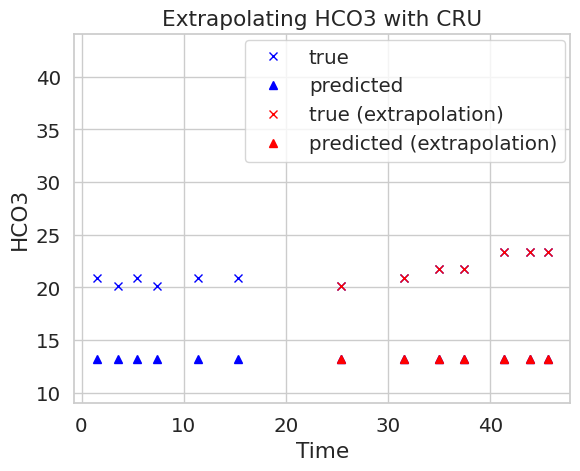
\includegraphics[width=0.45\linewidth]{content/chapters/irregular_time_series_data_driven_missingness/figures/true_vs_predicted_HCO3_cru.png} & 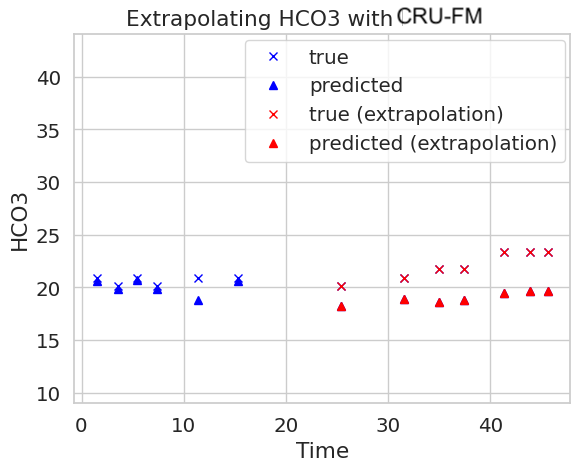
\includegraphics[width=0.45\linewidth]{content/chapters/irregular_time_series_data_driven_missingness/figures/true_vs_predicted_HCO3_mnar_cru.png} \\
        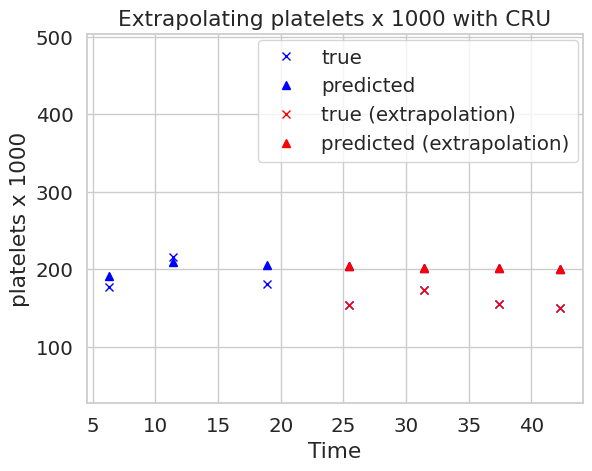
\includegraphics[width=0.45\linewidth]{content/chapters/irregular_time_series_data_driven_missingness/figures/true_vs_predicted_platelets_cru.png} & 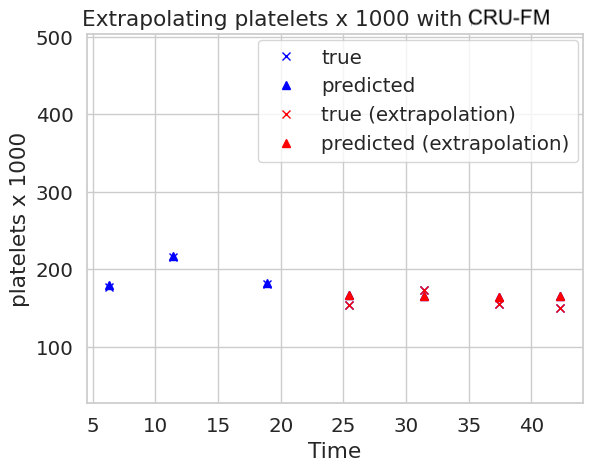
\includegraphics[width=0.45\linewidth]{content/chapters/irregular_time_series_data_driven_missingness/figures/true_vs_predicted_platelets_mnar_cru.png} \\
        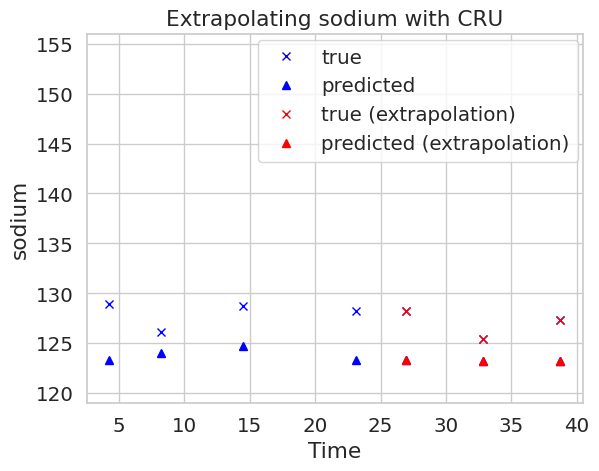
\includegraphics[width=0.45\linewidth]{content/chapters/irregular_time_series_data_driven_missingness/figures/true_vs_predicted_sodium_cru.png} & 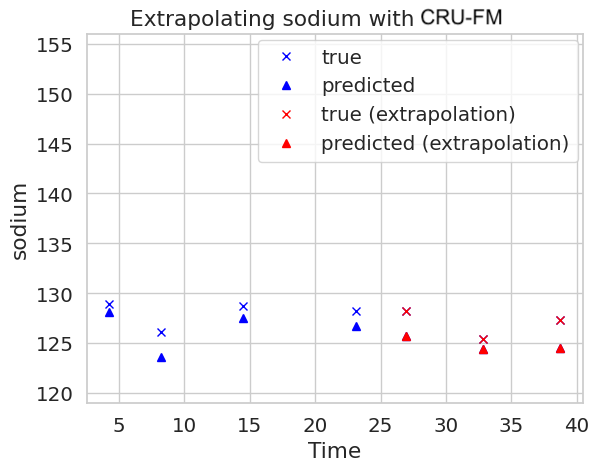
\includegraphics[width=0.45\linewidth]{content/chapters/irregular_time_series_data_driven_missingness/figures/true_vs_predicted_sodium_mnar_cru.png} \\
    \end{tabular}
    \caption{Illustrative examples of predicted trajectories from the eICU dataset, demonstrating that our CRU-FM outperforms the CRU in both extrapolation and interpolation of sequences.} 
    \label{fig:example_extrapolation_eICU} 
\end{figure}

\paragraph{Alternative method: CRU for concatenation of features and missingness mask.}
To confirm that improvements in our model stem from its ability to learn the mechanism of missing data, we introduced another baseline in which the missingness indicator mask $s_t$ is incorporated into the CRU as extra input feature channels. 
Below, we report results comparing our CRU-FM with the vanilla CRU with both features and missingness masks as inputs.

\begin{table}[ht]
\centering
\label{tab:cru_fm_vs_cru_w_mask}
\begin{tabular}{lcc}
\toprule
Lab Measurement & CRU-FM (test RMSE) & CRU w/ missing mask (test RMSE) \\ 
\midrule
creatinine & \textbf{0.86 (0.85, 0.89) }& 1.25 (1.22, 1.29) \\
potassium & \textbf{0.30 (0.29, 0.30)} & 0.38 (0.36, 0.41) \\
Sodium & \textbf{1.55 (1.52, 1.57)} & 1.77 (1.70, 1.82) \\
Platelets x 1000 & \textbf{89.86 (87.53, 92.22)} & 91.75 (89.66, 93.29) \\
Glucose & \textbf{46.81 (45.00, 48.63)} & 53.66 (53.10, 55.15) \\
HCO3 & \textbf{5.02 (4.92, 5.12)} & 6.01 (5.88, 6.18) \\
paO2 & \textbf{64.16 (63.00, 66.78)} & 73.22 (69.04, 77.21) \\
albumin & \textbf{0.44 (0.42, 0.49)} & 0.51 (0.48, 0.53) \\
ALT & \textbf{625.80 (584.00, 657.63)} & 696.52 (688.74, 705.81) \\
AST & \textbf{1148.96 (1100.80, 1200.86)} & 1248.19 (1236.01, 1271.91) \\
Bilirubin & \textbf{3.03 (2.75, 3.19)} & 3.80 (3.65, 3.84) \\
Troponin & 1.41 (1.27, 1.48) & \textbf{1.31 (1.20, 1.44) }\\
\bottomrule
\end{tabular}
\caption[Test RMSE of CRU (w/missing mask as input) and our CRU-FM on eICU dataset]{Comparing Test RMSE of CRU (w/missing mask as input) and our CRU-FM on the eICU dataset. In 11 out of 12 channels, our proposed method does better in terms of test RMSE.}
\end{table}


\paragraph{Predicting future missingness of a channel.} 
We additionally conduct  an experiment on the eICU and MIMIC-IV datasets assessing how jointly modeling features and missingness can predict future missingness of one particular channel (creatinine), chosen because it is infrequently observed and as a blood draw is likely to depend on data-driven decision-making. 
 
For each sequence in the test set :
	In interval $24h<t''<24h+w$ (window length) :
		Predict $s_{t'', creatinine} \in \{0, 1\}$ (predict if a measurement will be observed)

We trained a linear classifier (L2-penalized logistic regression) for 4 distinct scenarios that vary the input features fed into the classifier listed below:
\begin{itemize}
\item MCAR: input feature is just p, where p  is the patient-specific rate of observing a creatinine measurement in the first 24 hours (before the prediction interval)

\item Last observation only (MAR simple): classify $s_{t'', creatinine}|X_{obs},t'$, where $t'\in \mathbb{R}^D$ and $X_{obs}$, $t'\in \mathbb{R}^D$ is the last observed time point and measurement for each channel before 24 hours.

\item Modeling features only (MAR CRU) : classify $s_{t'', creatinine}|\mu_{t'_{24}}$ , where $\mu_{t'_{24}}$ refers to the representation vector  at time t=24 produced by the CRU model.

\item Modeling features + missingness (MAR CRU-FM) : classify $s_{t''}, creatinine|\mu_{t_{24}}$, where $\mu_{t_{24}}$ refers to the representation vector  at time t=24 produced by our model
\end{itemize}

Below for each model and possible window length, we report AUROC intervals computed from 100 bootstrapped samples on test set. % for various window lengths.

\begin{table}[ht]
\centering
\label{tab:missingness_classification_experiement}
\resizebox{.95\textwidth}{!}{
\begin{tabular}{llcccc}
\toprule
Dataset & Window Len. & MCAR & MAR Simple & MAR CRU & MAR CRU-FM \\ 
\midrule
\multirow{3}{*}{eICU} & 2 hours & 0.61 (0.57, 0.62) & 0.61 (0.59, 0.61) & 0.64 (0.63, 0.66) & \textbf{0.70 (0.69, 0.72)} \\
                      & 4 hours & 0.62 (0.58, 0.63) & 0.62 (0.60, 0.62) & 0.65 (0.63, 0.67) & \textbf{0.72 (0.70, 0.75)} \\
                      & 6 hours & 0.64 (0.60, 0.64) & 0.64 (0.62, 0.65) & 0.68 (0.66, 0.69) & \textbf{0.73 (0.71, 0.74)} \\
\hline
\multirow{3}{*}{MIMIC-IV} & 2 hours & 0.64 (0.63, 0.66) & 0.65 (0.63, 0.66) & 0.67 (0.66, 0.69) & \textbf{0.72 (0.69, 0.73)} \\
                          & 4 hours & 0.67 (0.64, 0.69) & 0.67 (0.66, 0.67) & 0.69 (0.68, 0.70) & \textbf{0.74 (0.70, 0.74)} \\
                          & 6 hours & 0.70 (0.69, 0.72) & 0.68 (0.66, 0.69) & 0.69 (0.68, 0.71) & \textbf{0.75 (0.72, 0.76)} \\
\bottomrule
\end{tabular}
}%endresizebox
\caption[Performance comparison for predicting future missingness of a channel]{The table presented above clearly illustrates the superiority of our model's approach—utilizing our CRU-FM’s representation vector for predicting the likelihood of a measurement occurring within a specified window, yields better AUROC compared to the alternative methods of relying solely on past observations or the simplistic strategy of utilizing a patient-specific observation rate (MCAR). Additionally, the improvement in AUROC as the window length increases can be attributed to the increase in ground truth positives.}
\end{table}

\paragraph{Extrapolation performance on extended list of channels}
In figure \ref{fig:all_channels_evaluation_extended}, we report the extrapolation performance on an extended list of channels beyond those reported in figure \ref{fig:real_data_evaluation}.
\begin{table*}[!tp]
    \centering
    \begin{tabular}{|l |c|}
        \hline        \rotatebox{90}{\hspace{3em}MIMIC-IV} 
        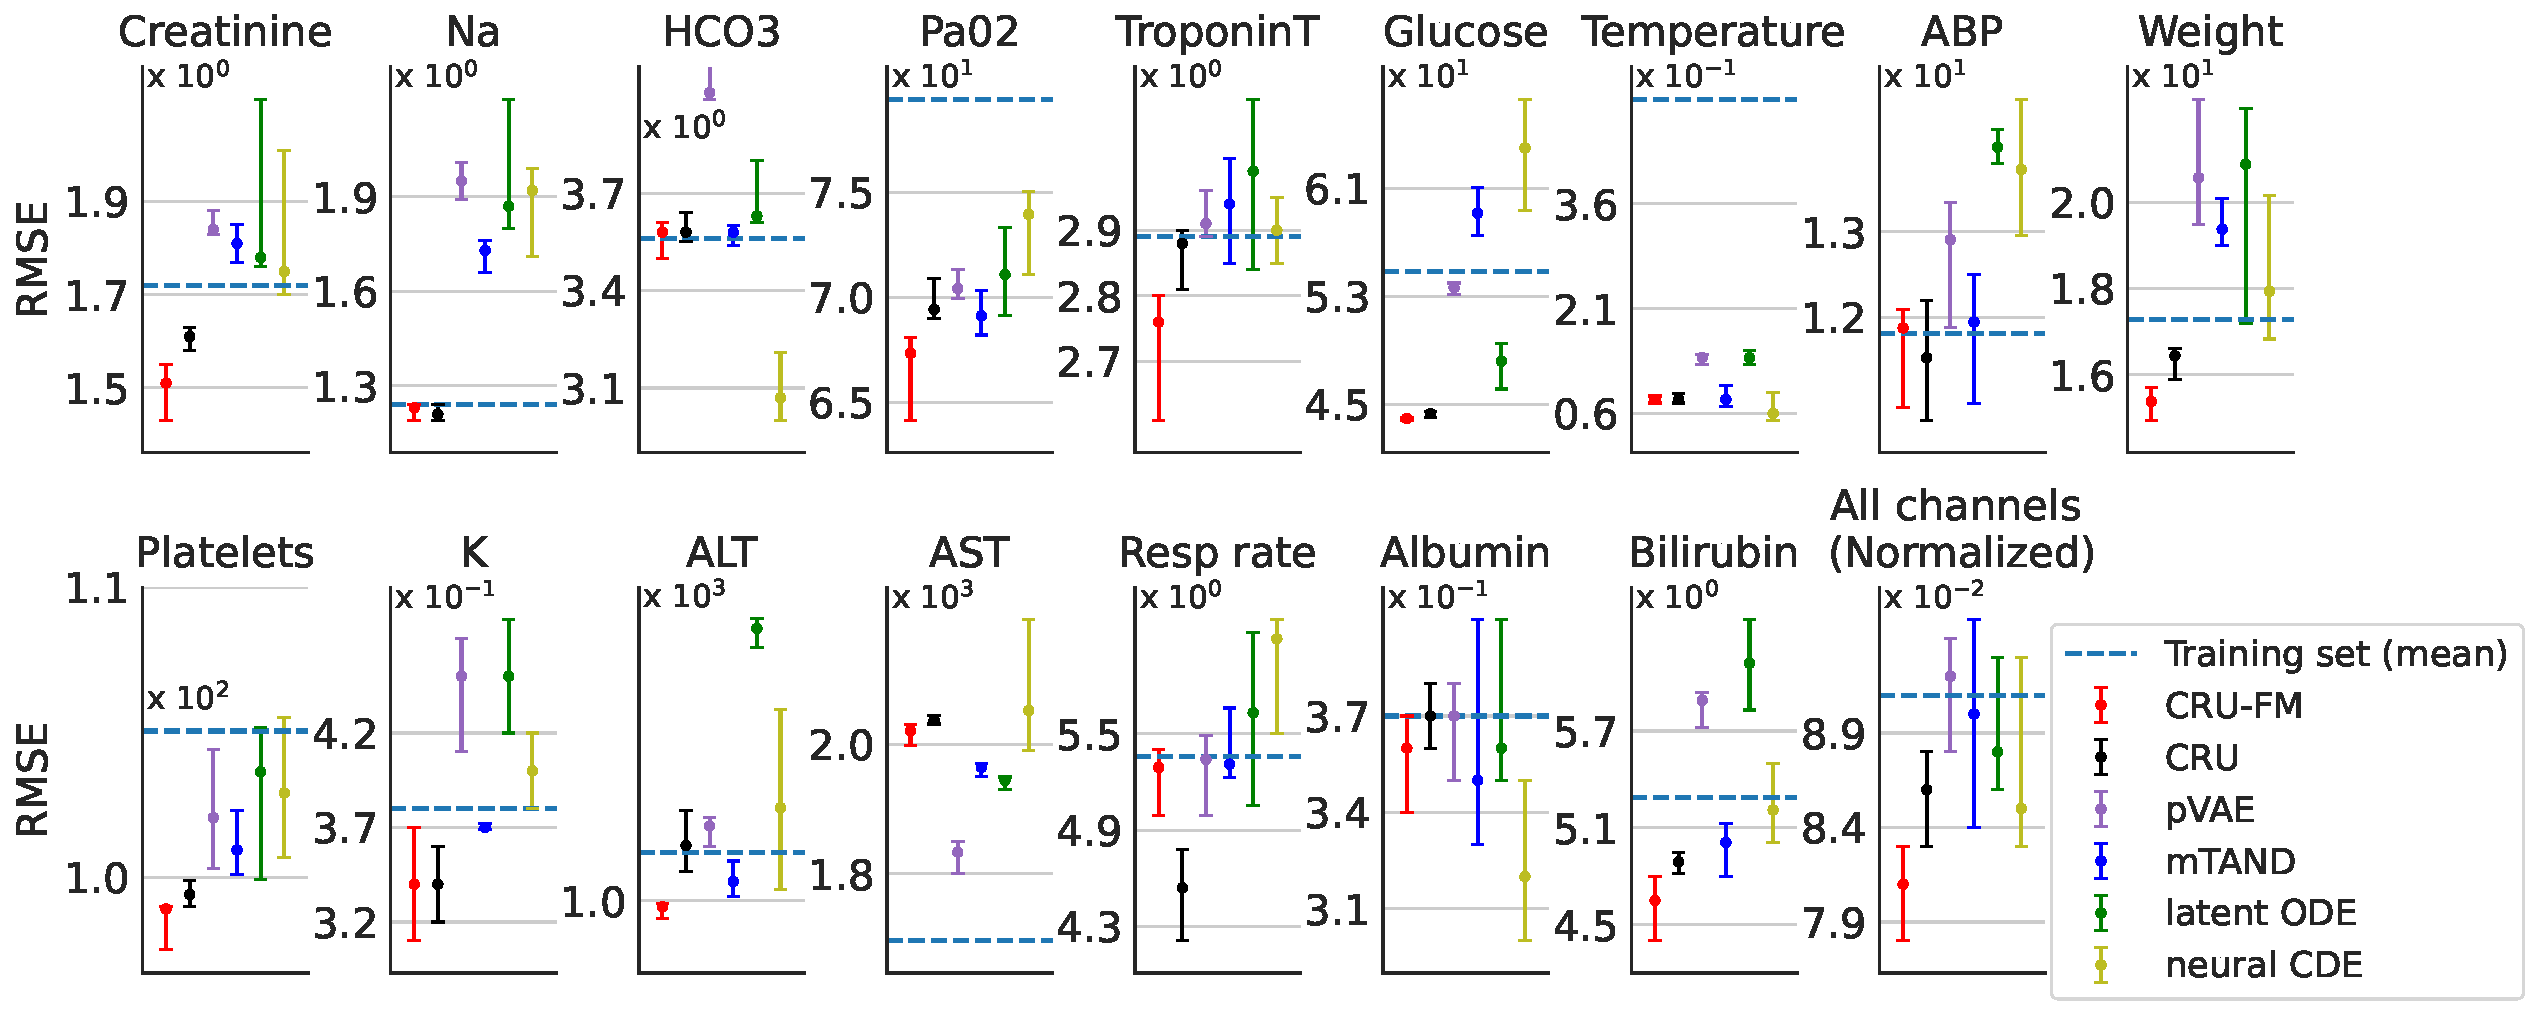
\includegraphics[width=0.95\textwidth]{content/chapters/irregular_time_series_data_driven_missingness/figures/mimic_evaluation.pdf} 
        \\~\\
        \hline
        \rotatebox{90}{\hspace{4em} Physionet} 
        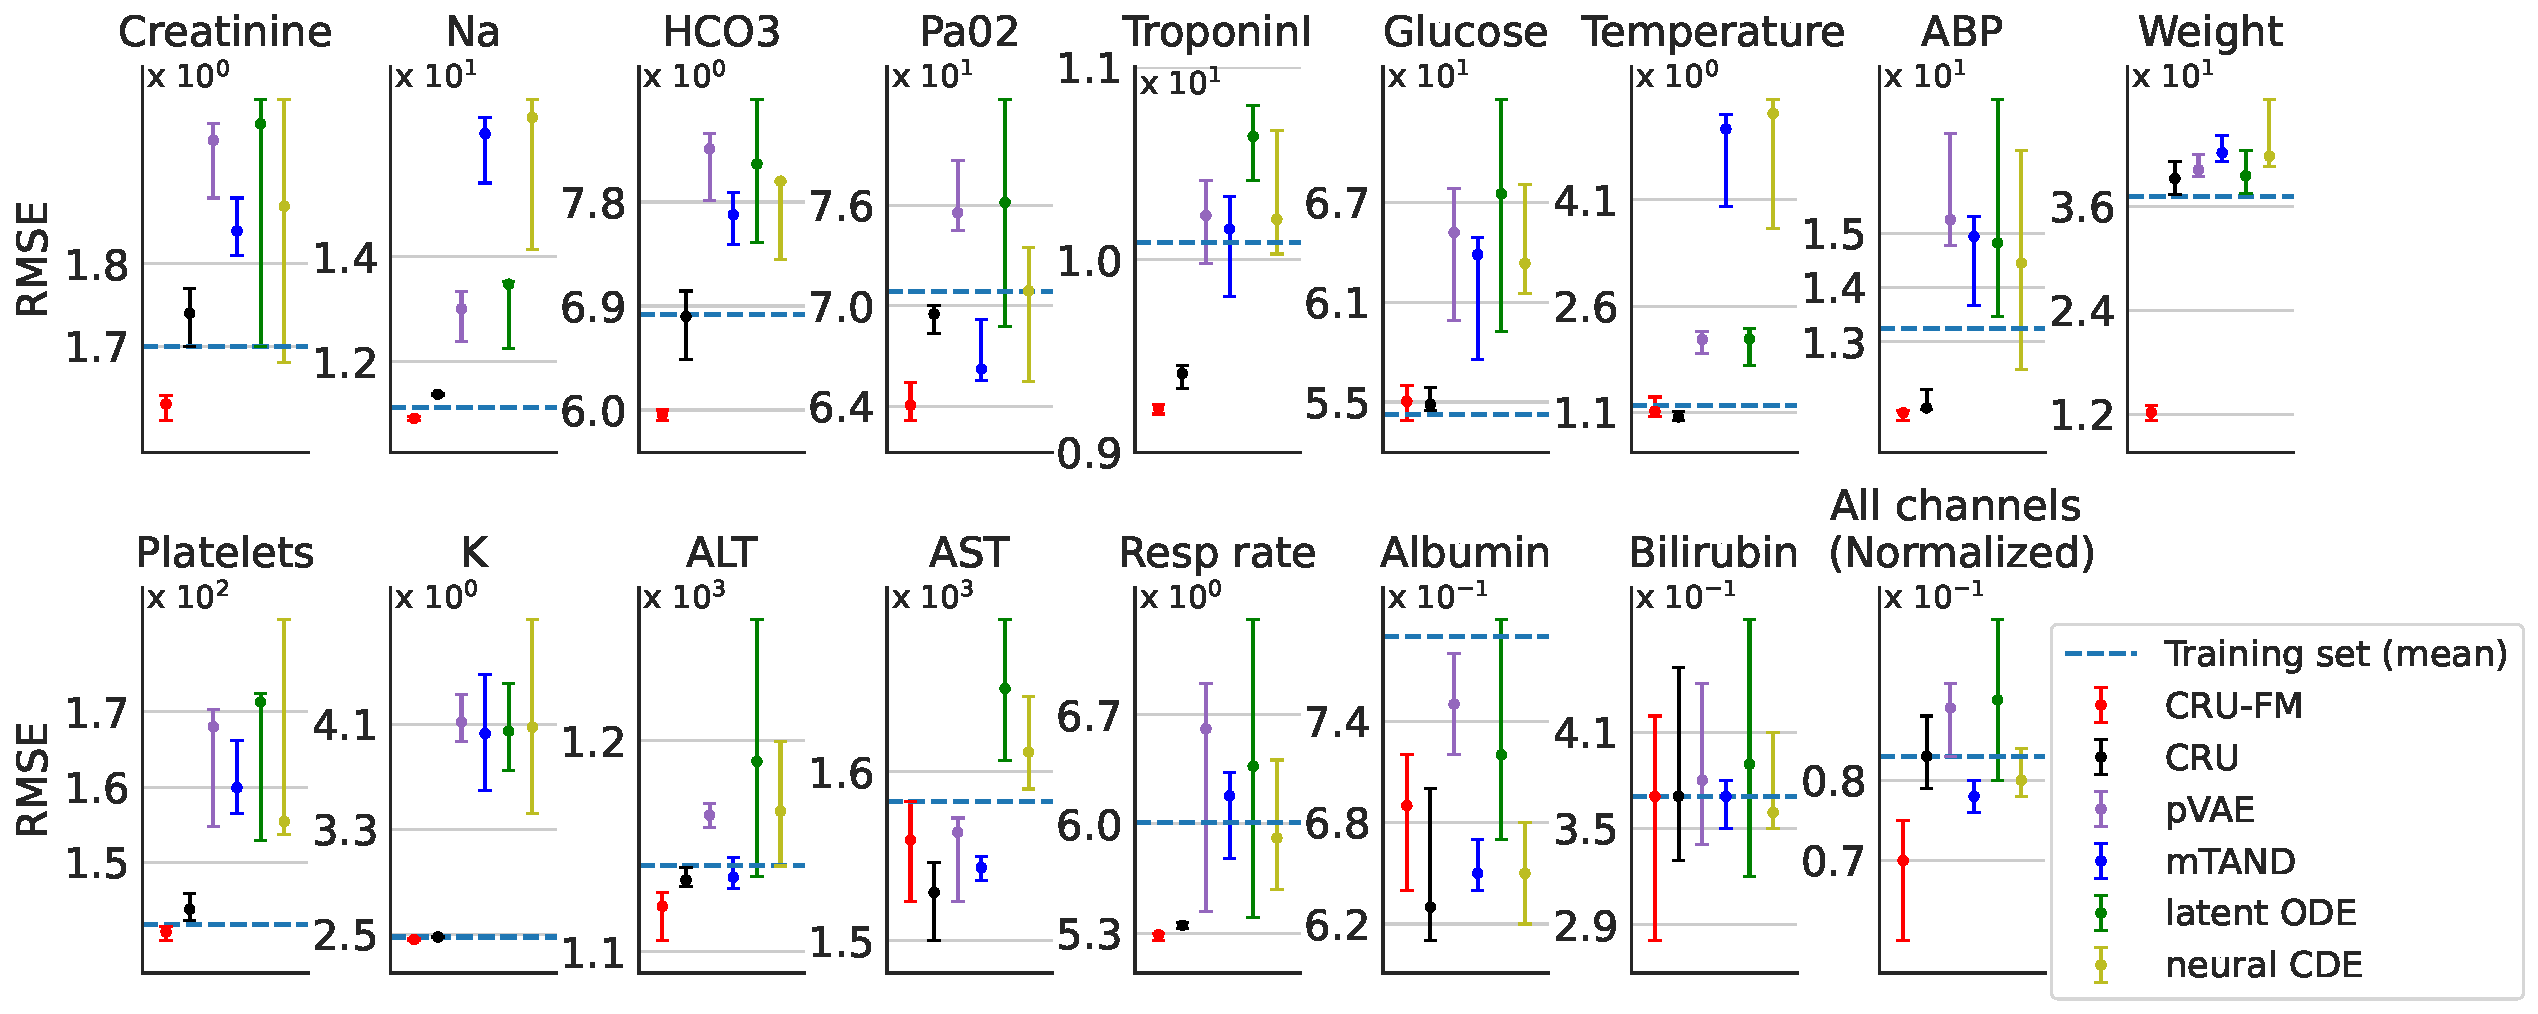
\includegraphics[width=0.95\textwidth]{content/chapters/irregular_time_series_data_driven_missingness/figures/physionet_evaluation.pdf} 
        \\~\\
        \hline
        \rotatebox{90}{\hspace{4em} eICU}
        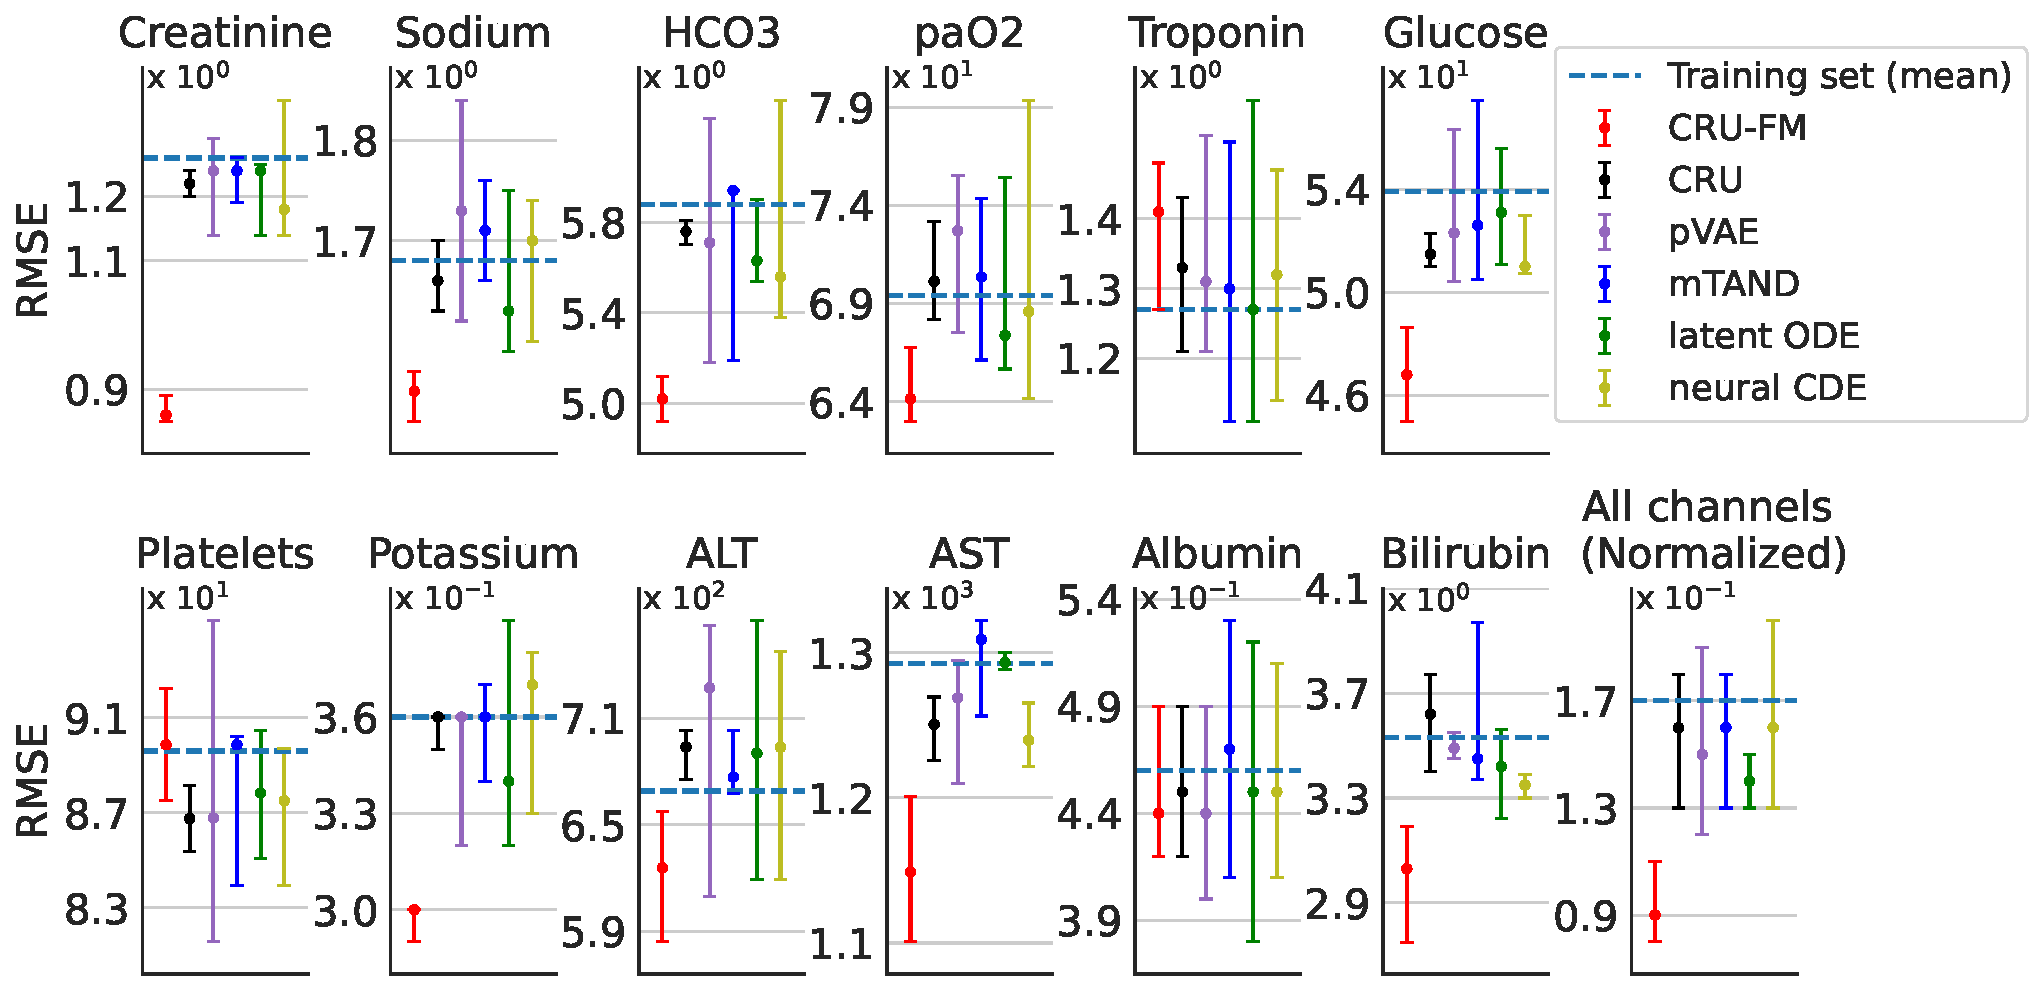
\includegraphics[width=0.95\textwidth]{content/chapters/irregular_time_series_data_driven_missingness/figures/eicu_evaluation.pdf}\\
        \hline
    \end{tabular}
    \caption[Extrapolation performance on extended list of channels on 3 EHR datasets comparing 5 baselines with our CRU-FM]{RMSE comparison of our CRU-FM with 5 baselines after training on the first 24 hours of data and extrapolating the next 24 hours of measurements on MIMIC-4, Physionet, and eICU. Confidence intervals represent the 5th and 95th percentiles from 100 bootstrapped samples from the test set. Our CRU-FM outperforms baselines in 8/16 channels in MIMIC-4, 11/16 channels on Physionet and 7/12 channels in eICU (RMSE confidence intervals are lower and do not overlap with baselines). The training set mean baseline is added to uncover a gap in existing studies \citep{shukla2021multitime, rubanova2019latent}, which overlooked a simple yet effective benchmark that, while showing decent RMSE performance, falls short in complex clinical decision-making settings.}
    \label{fig:all_channels_evaluation_extended}
\end{table*}
